
% variational-autoencoder.tex

\documentclass[dvipdfmx,notheorems,t]{beamer}

\usepackage{docmute}

% settings.tex

\AtBeginDvi{\special{pdf:tounicode 90ms-RKSJ-UCS2}}

\AtBeginSection[]{\frame[t]{\frametitle{目次}
	\tableofcontents[currentsection,hideallsubsections]}}

\AtBeginSubsection[]{\frame[t]{\frametitle{目次}
	\tableofcontents[currentsection,currentsubsection,subsectionstyle=show/shaded/hide]}}

\usefonttheme{professionalfonts}
\usetheme{Madrid}

\setbeamercovered{transparent=30} 
% \setbeamertemplate{navigation symbols}{}
\setbeamertemplate{frametitle}[default][left]
\setbeamertemplate{frametitle continuation}{}
\setbeamertemplate{enumerate items}[square]
\setbeamertemplate{caption}[numbered]

\let\oldframe\frame
\renewcommand\frame[1][allowdisplaybreaks,allowframebreaks,t]{\oldframe[#1]}

\usepackage{bxdpx-beamer}
\usepackage{pxjahyper}
\usepackage{minijs}

\usepackage{amsmath}
\usepackage{amssymb}
\usepackage{amsthm}
\usepackage{bm}

\DeclareMathOperator*{\argmax}{arg\,max}
\DeclareMathOperator*{\argmin}{arg\,min}
\DeclareMathOperator{\Tr}{Tr}
\DeclareMathOperator{\KL}{KL}
\DeclareMathOperator{\diag}{diag}

\usepackage[T1]{fontenc}
\usepackage[utf8]{inputenc}

\setbeamertemplate{theorems}[numbered]
\theoremstyle{definition}
\newtheorem{theorem}{定理}
\newtheorem{definition}{定義}
\newtheorem{proposition}{命題}
\newtheorem{lemma}{補題}
\newtheorem{corollary}{系}
\newtheorem{conjecture}{予想}
\newtheorem*{remark}{Remark}
\renewcommand{\proofname}{}

\renewcommand{\figurename}{図}
\renewcommand{\tablename}{表}

\renewcommand{\kanjifamilydefault}{\gtdefault}


\begin{document}

\section{変分自己符号化器}

\subsection{生成モデル}

\begin{frame}{生成モデル}

\begin{itemize}
	\item 生成モデルの目的
	\begin{itemize}
		\item データ$\bm{x}$に関する分布$p(\bm{x})$を推定する
	\end{itemize} \
	
	\item データ生成過程
	\begin{itemize}
		\item データ$\bm{x}$は一般に高次元である
		\item 但し、実際にデータが分布しているのは、ごく限られた一部の低次元の領域であると考えられる (\alert{多様体仮説})
		\item データ$\bm{x}$自体は高次元だが、本質的には低次元の情報しか持たないと考えられる
		\newline
		
		\item データ$\bm{x}$を、より低次元なベクトル$\bm{z}$を使って、表現することを考える
		\item データに関する分布$p(\bm{x})$を、潜在変数$\bm{z}$に関する分布と、うまく組み合わせて記述する
		\item \alert{潜在変数からデータが生成されるまでの過程}を組み込んで、$p(\bm{x})$を記述する
	\end{itemize}
\end{itemize}

\end{frame}

\subsection{変分自己符号化器(VAE)の概要}

\begin{frame}{変分自己符号化器(VAE)の概要}

\begin{itemize}
	\item 深層学習における生成モデル
	\begin{itemize}
		\item 主に以下の2つの手法が存在する
		\newline
		
		\item 敵対的生成ネットワーク (Generative Adversarial Networks, GAN)
		\item \alert{変分自己符号化器} (Variational Auto Encoders, \alert{VAE})
		\newline
		
		\item ここでは変分自己符号化器(VAE)について扱う
		\newline
		
		\item VAEを、異常検知(不良品の検出など)に使った例がある
	\end{itemize}
\end{itemize}

\end{frame}

\begin{frame}{変分自己符号化器(VAE)の概要}

\begin{itemize}
	\item VAEにおけるグラフィカルモデル
	\begin{itemize}
		\item 図\ref{fig:vae-graphical-model}のような、潜在変数を含んだグラフィカルモデルを考える
		\newline
		
		\item データ$\bm{x}$について、ある一つの潜在変数$\bm{z}$が対応しているとする
		\item 各データ$\bm{x}$は、分布$p(\bm{x})$から独立にサンプルされるとする
		\item 従って、データ$\left\{ \bm{x}_1, \ldots, \bm{x}_N \right\}$は\alert{独立同分布標本}とする
		\newline
		
		\item $\theta$は、\color{red}潜在変数$\bm{z}$からデータ$\bm{x}$\normalcolor を取得する際に使用されるパラメータ
		\item $\phi$は、\color{red}データ$\bm{x}$から潜在変数$\bm{z}$\normalcolor を生成する際に使用されるパラメータ
		\item $N$は、データ数である
	\end{itemize}
\end{itemize}

\end{frame}

\begin{frame}{変分自己符号化器(VAE)の概要}

\begin{itemize}
	\item データ$\bm{x}$の生成過程
	\begin{itemize}
		\item データ$\bm{x}$の生成過程は、次のように考える
		\newline
		\item 分布\color{red}$p(\bm{z} | \theta)$\normalcolor から、潜在変数$\bm{z}_i$がサンプルされる
		\item 分布\color{red}$p(\bm{x} | \bm{z}_i, \theta)$\normalcolor から、データ$\bm{x}_i$がサンプルされる
		\newline
		
		\item これより、データ$\bm{x}$の分布を次のように表現できる
		\begin{equation}
			p(\bm{x} | \theta) = \int p(\bm{x} | \bm{z}, \theta) p(\bm{z} | \theta) d\bm{z}
		\end{equation}
	\end{itemize} \
	
	\item 潜在変数$\bm{z}$をデータ$\bm{x}$から取得する過程
	\begin{itemize}
		\item 潜在変数$\bm{z}_i$をデータ$\bm{x}_i$から得る過程は、次のように考える
		\newline
		\item 分布\color{red}$q(\bm{z} | \bm{x}_i, \phi)$\normalcolor から、潜在変数$\bm{z}_i$がサンプルされる
	\end{itemize}
\end{itemize}

\end{frame}

\begin{frame}{変分自己符号化器(VAE)の概要}

\begin{figure}
	\centering
	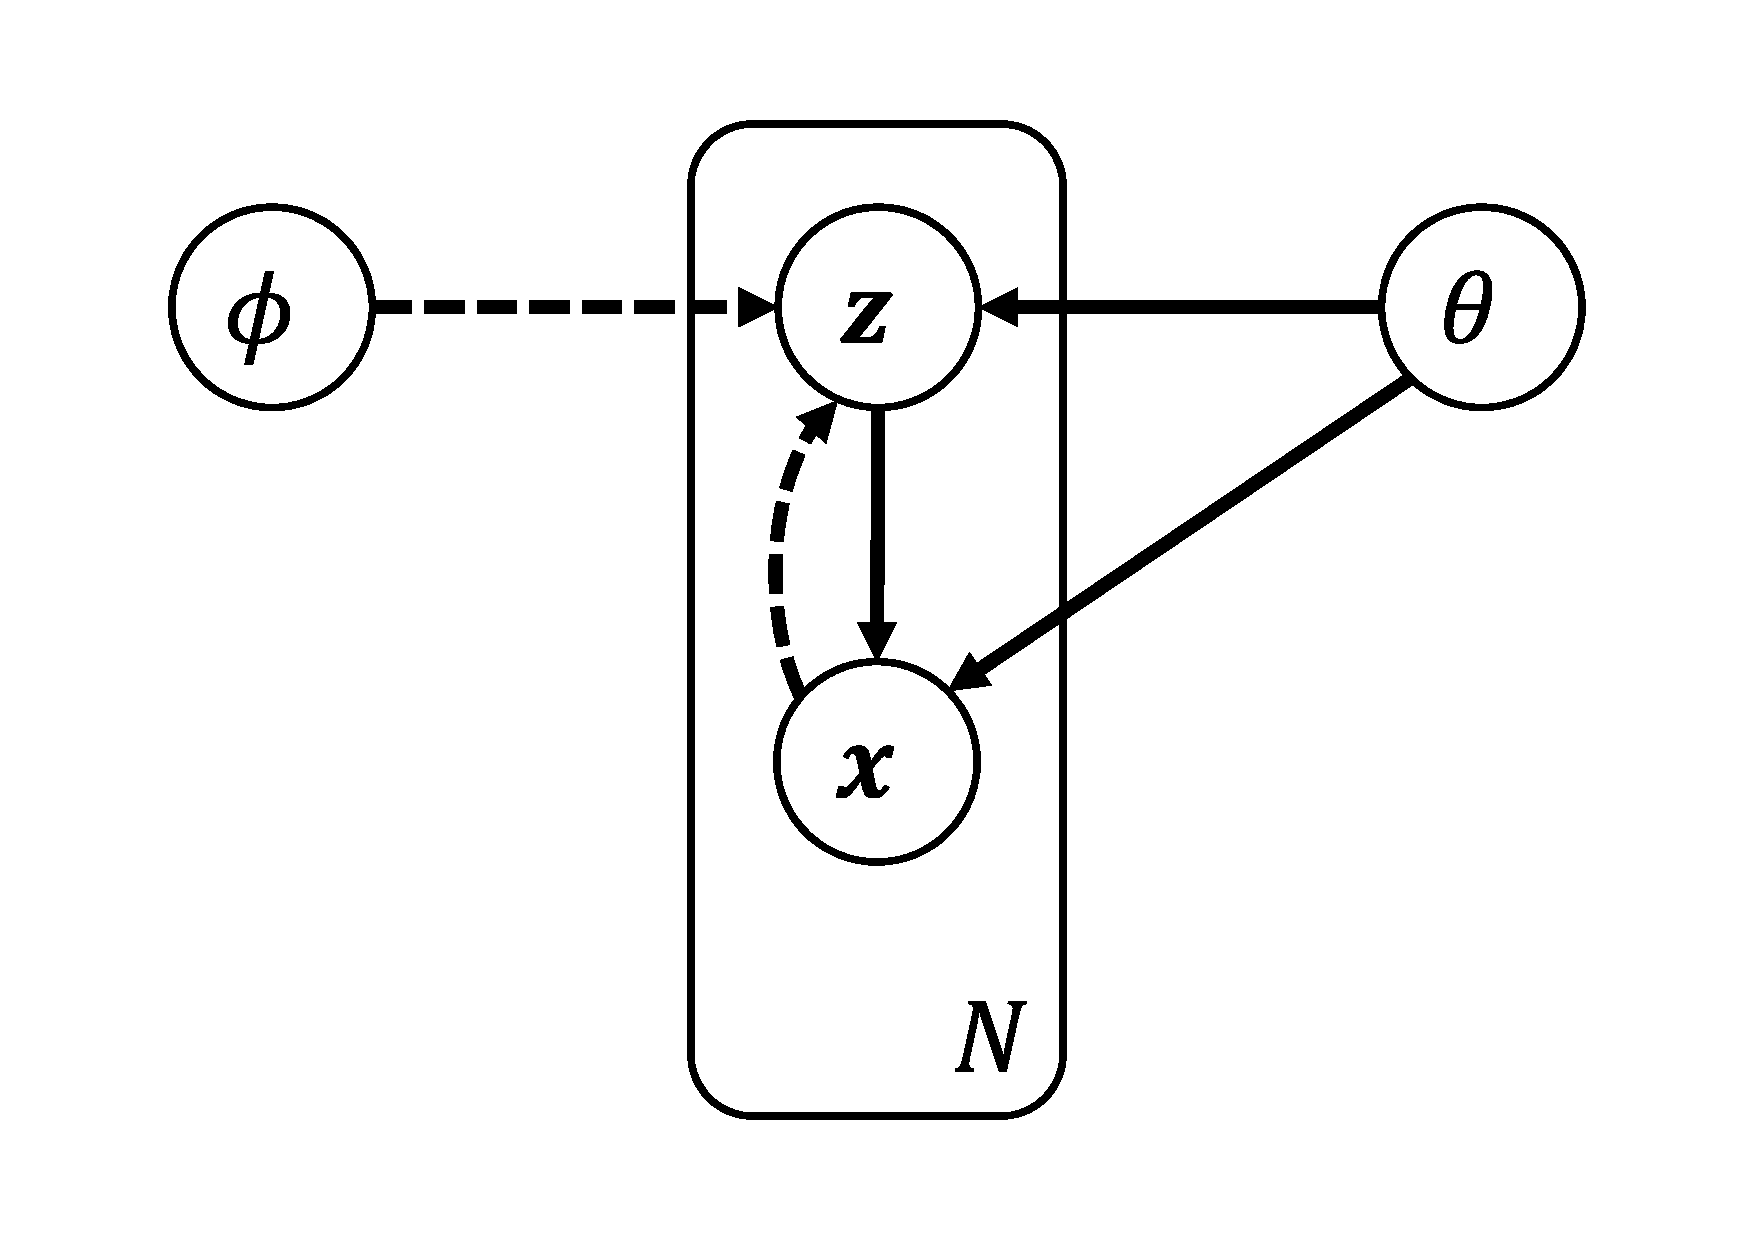
\includegraphics[keepaspectratio,scale=0.2]{vae-graphical-model.pdf}
	\caption{変分自己符号化器(VAE)におけるグラフィカルモデル}
	\label{fig:vae-graphical-model}
\end{figure}

\end{frame}

\begin{frame}{変分自己符号化器(VAE)の概要}

\begin{itemize}
	\item 確率分布のニューラルネットワークによる表現
	\begin{itemize}
		\item 潜在変数を含む確率モデルについて、パラメータの最尤解を求めるために、EMアルゴリズムを導出した
		\item EMアルゴリズムでは、潜在変数に関する事後分布$p(\bm{z} | \bm{x}, \theta)$を計算する必要があった
		\item この事後分布$p(\bm{z} | \bm{x}, \theta)$の計算が困難であるとき、$p(\bm{z} | \bm{x}, \theta)$を別の分布$q(\bm{z} | \bm{x}, \phi)$で近似し、変分推論によって$q(\bm{z} | \phi)$の最適解を求めた
		\newline
		\item VAEは変分推論の変種であり、近似事後分布$q(\bm{z} | \bm{x}, \phi)$と、$p(\bm{x} | \bm{z}, \theta)$の2つを\alert{ニューラルネットワーク}で表現する
		\newline
		\item データ$\bm{x}$を潜在変数$\bm{z}$に対応付けるニューラルネットワークを、\alert{Encoder}という
		\item 潜在変数$\bm{z}$からデータ$\bm{x}$を復元するニューラルネットワークを、\alert{Decoder}という
		\item 分布$q(\bm{z} | \bm{x}, \phi)$は\alert{Encoder}、分布$p(\bm{x} | \bm{z}, \theta)$は\alert{Encoder}に相当する
	\end{itemize}
\end{itemize}

\end{frame}

\subsection{変分自己符号化器(VAE)の理論}

\begin{frame}{変分自己符号化器(VAE)の理論}

\begin{itemize}
	\item 変分自己符号化器(VAE)の理論
	\begin{itemize}
		\item 変分下界$\mathcal{L}(q)$は次のようであった
		\begin{eqnarray}
			\mathcal{L}(q) &=& \int q(\bm{z} | \bm{x}) \ln \frac{p(\bm{x}, \bm{z})}{q(\bm{z} | \bm{x})} d\bm{z} \\
			&=& \int q(\bm{z}) \ln \frac{p(\bm{x} | \bm{z}) p(\bm{z})}{q(\bm{z} | \bm{x})} d\bm{z} \\
			&=& \int q(\bm{z} \ln p(\bm{x} | \bm{z}) d\bm{z} + \int q(\bm{z} | \bm{x}) \ln \frac{p(\bm{z})}{q(\bm{z} | \bm{x})} d\bm{z} \\
			&=& \int q(\bm{z}) \ln p(\bm{x} | \bm{z}) d\bm{z} - \KL(q(\bm{z} | \bm{x}) || p(\bm{z})) \\
			&=& \mathbb{E}_{\bm{z} \sim q(\bm{z})} \left[ \ln p(\bm{x} | \bm{z}) \right] - \KL(q(\bm{z} | \bm{x}) || p(\bm{z}))
		\end{eqnarray}
		
		\item ここでは、単一のデータ$\bm{x}$と、それに対応する潜在変数$\bm{z}$を考えている
		\newline
		
		\item KLダイバージェンスの項は、後ほど求めることにする(解析的に求められる)
		\item 第1項は、分布$q(\bm{z})$に関する期待値であり、VAEでは\alert{サンプリングで近似}する
		\begin{equation}
			\mathbb{E}_{\bm{z} \sim q(\bm{z})} \left[ \ln p(\bm{x} | \bm{z}) \right] \simeq \frac{1}{L} \sum_{i = 1}^L \ln p(\bm{x}_i | \bm{z}_{i, l})
		\end{equation}
		
		\item これより、変分下界$\mathcal{L}(q)$は以下のように書ける
		\begin{equation}
			\mathcal{L}(q) \simeq -\KL(q(\bm{z} | \bm{x}) || p(\bm{z})) + \frac{1}{L} \sum_{i = 1}^L \ln p(\bm{x}_i | \bm{z}_{i, l})
		\end{equation}
	\end{itemize}
\end{itemize}

\end{frame}

\end{document}
